\section*{CHƯƠNG 3: TẠO THƯ VIỆN SCHEMATIC VÀ FOOTPRINT}
\stepcounter{section}
\addcontentsline{toc}{section}{\numberline{}CHƯƠNG 3: TẠO THƯ VIỆN SCHEMATIC VÀ FOOTPRINT}
\subsection{Trình tự tạo thư viện schematic}
Bước 1: Chọn File/New/Library để tạo thư viện mới.
\begin{figure}[H]
    \centering
    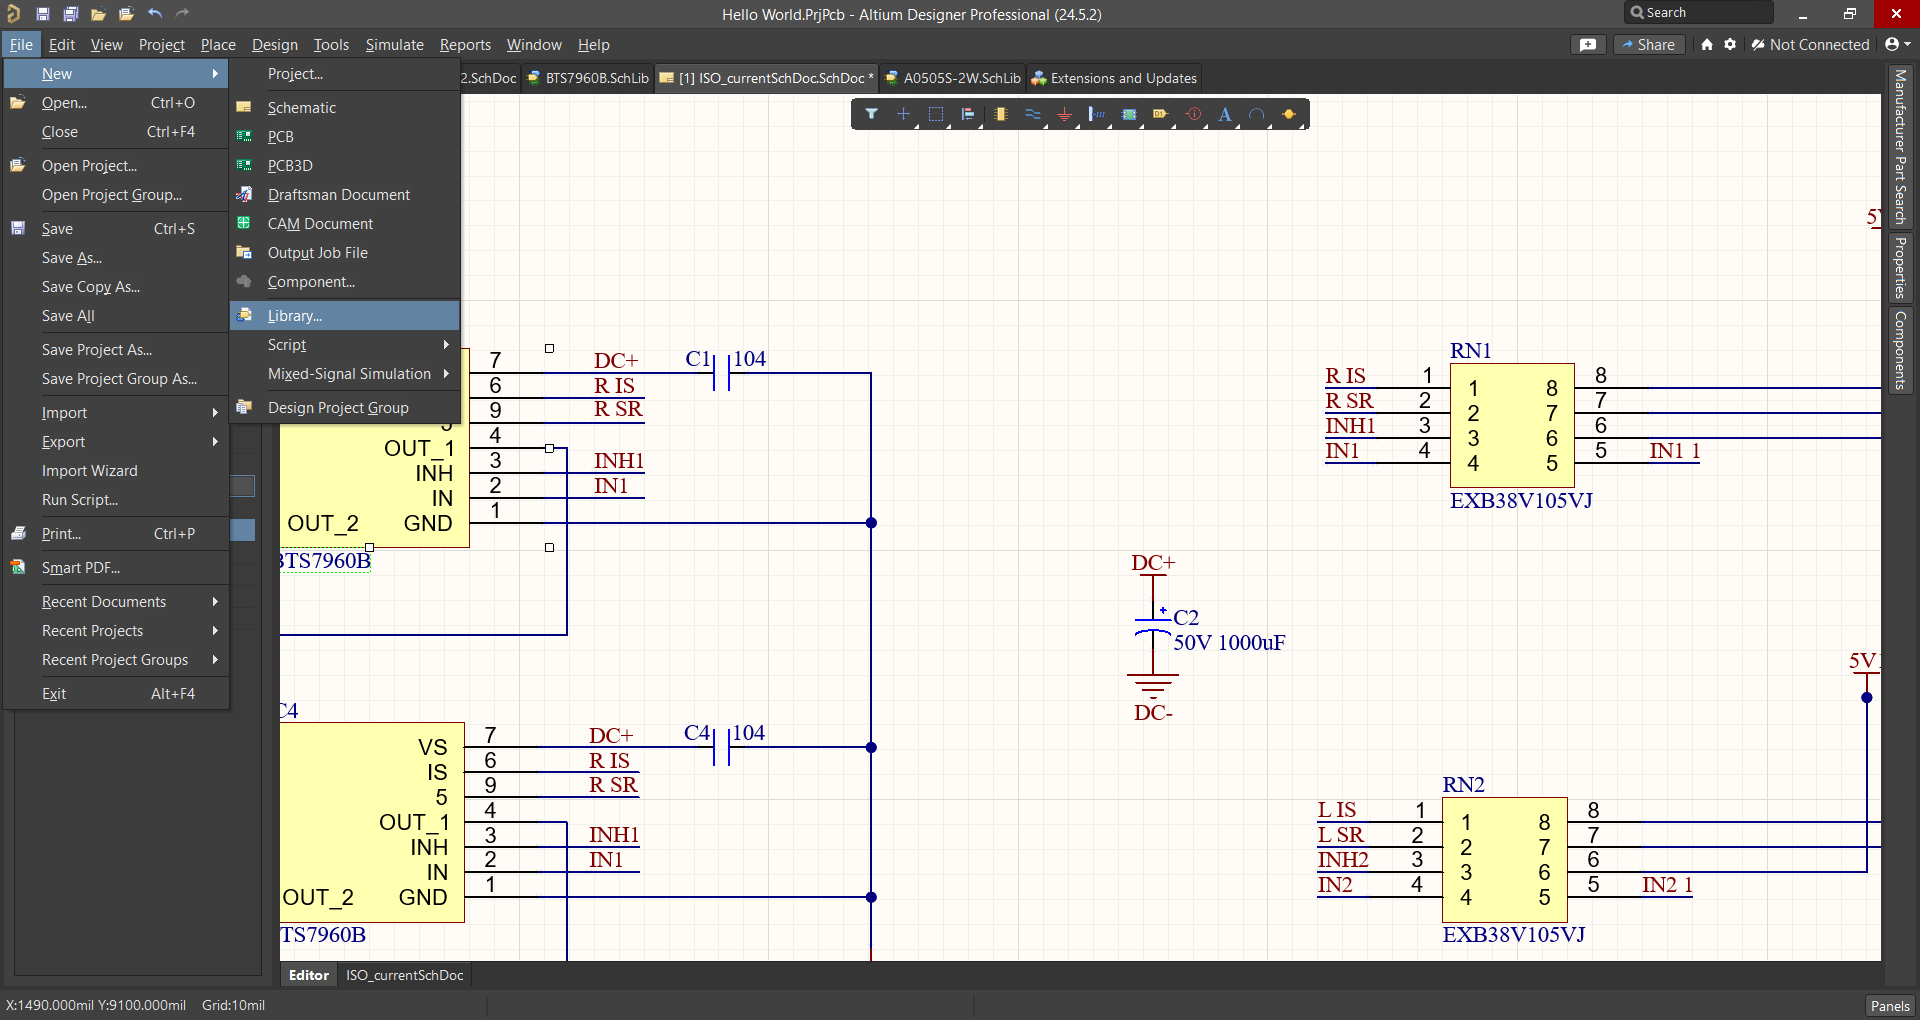
\includegraphics[width=1\textwidth]{image/ch3.1.png}
    \caption{Tạo thư viện schematic mới bước 1}
\end{figure}
Bước 2: Chọn Schematic Library và nhấn Create.
\begin{figure}[H]
    \centering
    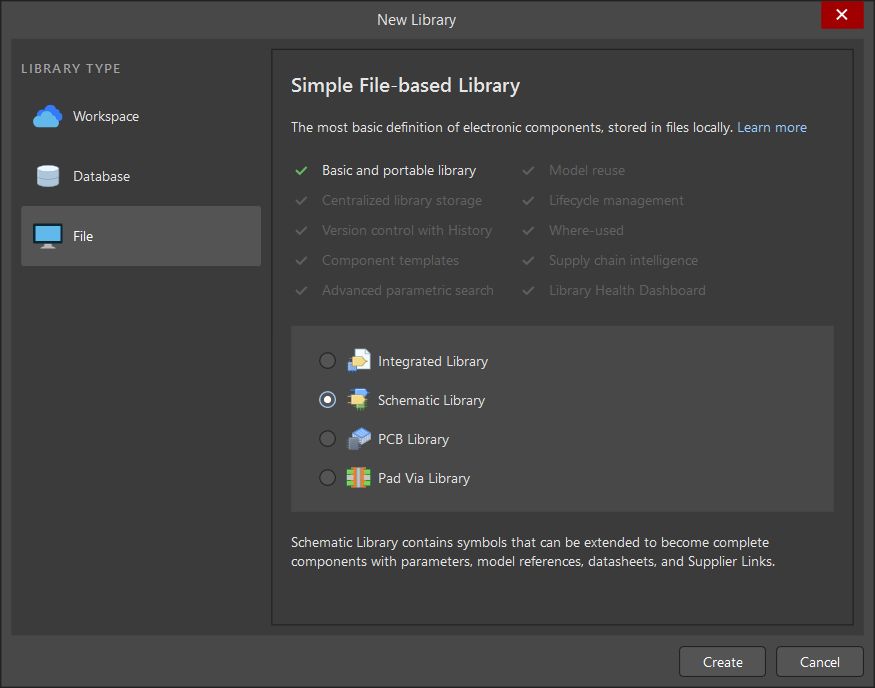
\includegraphics[width=1\textwidth]{image/ch3.2.png}
    \caption{Tạo thư viện schematic mới bước 2}
\end{figure}
Bước 3: Vẽ schematic theo nhu cầu.
\begin{figure}[H]
    \centering
    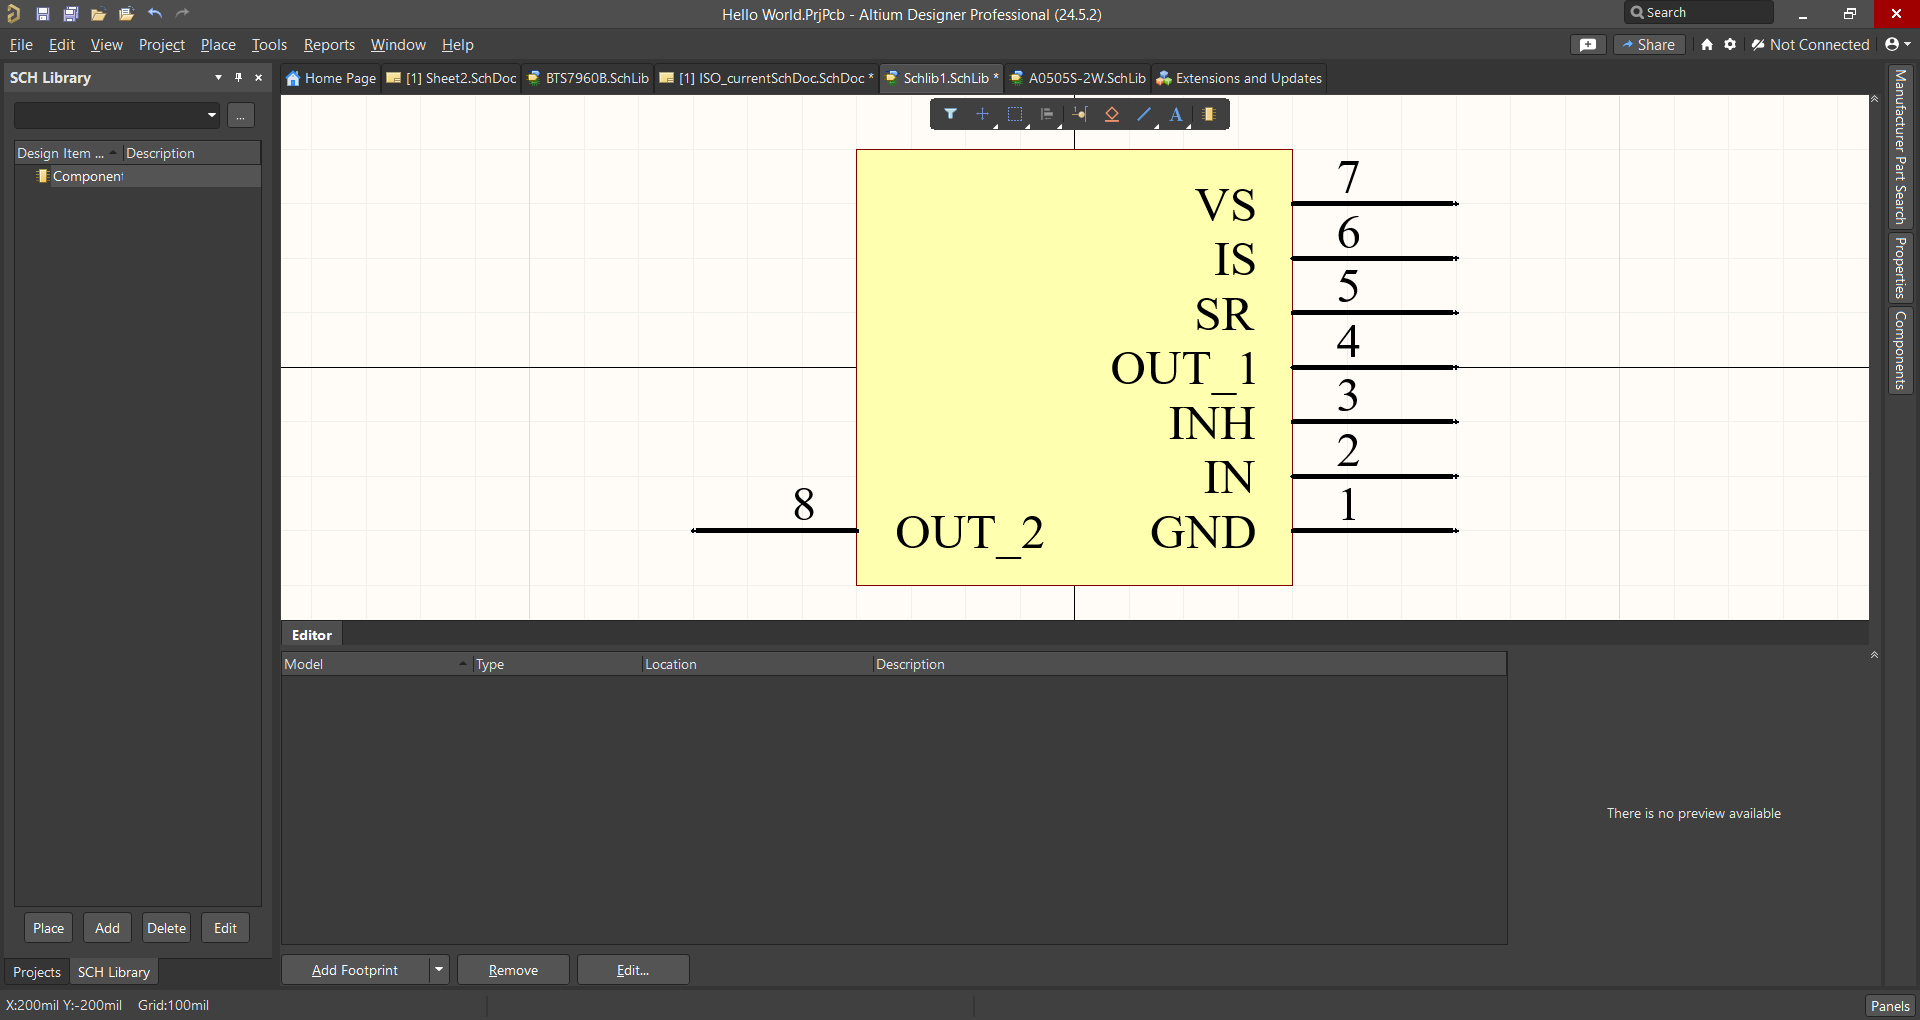
\includegraphics[width=1\textwidth]{image/ch3.3.png}
    \caption{Tạo thư viện schematic mới bước 3}
\end{figure}
Bước 4: Đặt tên cho thư viện và lưu lại.\\
Bước 5:
\cleardoublepage